
\documentclass[twoside]{ctuthesis}

\ctusetup{
	% preprint = \today,
	mainlanguage = english,
	otherlanguages = {czech},
	title-czech = {Gamifikace ve výuce anglických slovíček},
	title-english = {Gamification for English Vocabulary Learning},
	subtitle-czech = {},
	subtitle-english = {},
	doctype = B,
	faculty = F3,
	department-czech = {Katedra počítačové grafiky a interakce},
	department-english = {Department of Computer Graphics and Interaction},
	author = {Petr Nejedlý},
	supervisor = {Ing. Ivo Malý, Ph.D.},
	% supervisor-address = {KN:E-425, \\ Karlovo náměstí 13, \\ Praha 2},
	fieldofstudy-english = {Software Engineering and Technology},
	subfieldofstudy-english = {Business Informatics},
	fieldofstudy-czech = {Softwarové inženýrství a technologie},
	subfieldofstudy-czech = {Business Informatics},
	keywords-czech = {gamifikace, výuka anglických slovíček, mobilní aplikace, Flutter},
	keywords-english = {gamification, English vocabulary learning, mobile app, Flutter},
	day = 26,
	month = 12,
	year = 2024
%	specification-file = {ctutest-zadani.pdf},
%	front-specification = true,
%	front-list-of-figures = false,
%	front-list-of-tables = false,
%	monochrome = true,
%	layout-short = true,
}

\ctuprocess

\setlength{\parskip}{1em}

\addto\ctucaptionsczech{
	\def\supervisorname{Vedoucí}
	\def\subfieldofstudyname{Studijní program}
}

\ctutemplateset{maketitle twocolumn default}{
	\begin{twocolumnfrontmatterpage}
		\ctutemplate{twocolumn.thanks}
		\ctutemplate{twocolumn.declaration}
		\ctutemplate{twocolumn.abstract.in.titlelanguage}
		\ctutemplate{twocolumn.abstract.in.secondlanguage}
		\ctutemplate{twocolumn.tableofcontents}
		\ctutemplate{twocolumn.listoffigures}
	\end{twocolumnfrontmatterpage}
}

\begin{abstract-czech}
TODO: tady bude abstrakt v češtině ...
\end{abstract-czech}
    
\begin{abstract-english}
TODO: here will be an abstract in English
\end{abstract-english}
\begin{thanks}
I would like to express my sincere gratitude to my supervisor, \ctufield{supervisor}, for his guidance and constructive feedback throughout the development of this thesis.

I am also grateful to all the participants who took part in the user testing sessions, providing valuable insights that helped improve the application.

Special thanks go to my family and friends for their continuous support and understanding during the course of this project.
\end{thanks}
\begin{declaration}
TODO: Declaration...

In Prague,~\monthinlanguage{title} \ctufield{day},~\ctufield{year}
\end{declaration}

\begin{document}

\maketitle

% ----- CHAPTERS -----
\chapter{Introduction}

In today's fast-paced digital world, language learning applications have become an essential tool for individuals seeking to enhance their vocabulary and language skills. However, maintaining user engagement and motivation over time remains a significant challenge. This project addresses this issue by exploring the integration of gamification elements into the English Mind application, aiming to transform the learning experience into a more engaging and rewarding journey.

The English Mind application is built on a well-designed learning approach that effectively supports language acquisition. However, when compared to leading competitors, it falls short in terms of gamification elements. This lack of engaging features may negatively impact user motivation and retention, as users are increasingly drawn to applications that offer interactive and rewarding experiences. 

This project aims to address this gap by integrating gamification strategies that can enhance user engagement and motivation, thereby positioning English Mind more competitively in the market.

\newpage

\section{Success Criteria}

The evaluation of this work's success is structured around three principal dimensions: competitive positioning, user feedback, and implementation success. These dimensions serve as the foundation for assessing the achievement of the thesis objectives.

\begin{enumerate}
    \item \textbf{Enhancement of Competitive Positioning}
    \begin{enumerate}
        \item Analyze the English Mind vocabulary learning approach to understand the key principles of the application.
        \item Conduct analysis of gamification features used by English Mind and leading competitors.
        \item Identify opportunities for enhancing the gamification of English Mind.
    \end{enumerate}

    \item \textbf{Positive User Feedback on Gamification Features}
    \begin{enumerate}
        \item Design gamification features and elements that are on par with or surpass those of leading competitors.
        \item Conduct user testing of the new gamification features, aiming for positive feedback.
    \end{enumerate}

    \item \textbf{Successful Implementation of Gamification Features}
    \begin{enumerate}
        \item Implement the newly designed gamification features into the application.
        \item Conduct testing with end users to ensure functionality and user satisfaction.
    \end{enumerate}
\end{enumerate}

\chapter{Mobile Application English Mind}
\label{chap:mobile-application-english-mind}

English Mind is a mobile application available on Android \cite{cite:english_mind_play_store} and iOS \cite{cite:english_mind_app_store} platforms that focuses on learning English vocabulary. To achieve high efficiency in learning new English vocabulary, the application combines three main teaching methods on which it is based \cite{cite:english_mind_website}:

\begin{itemize}
    \item Frequency list of English vocabulary
    \item Active recall utilizing flashcards
    \item Spaced repetition system
\end{itemize}

These methods create a structured and efficient approach to mastering vocabulary with minimal effort, setting the app apart from its competitors in the field of vocabulary learning apps.

\section{Frequency List}

A frequency list ranks words according to their occurrence in common texts and speech. This approach is particularly valuable in vocabulary teaching for foreign language learners, as learning high-frequency words first enables students to comprehend more of their target language earlier in their studies.

Research by Nation \cite{cite:nation2006_how_large_vocabulary_is_needed} demonstrates the effectiveness of this approach. Mastering the 1,000 most frequent word families enables understanding of 78-81\% of written text, while 8,000-9,000 word families are required for 98\% comprehension. This data underscores the importance of prioritizing high-frequency vocabulary in language acquisition.\newpage

The frequency list implementation in English Mind allows users to browse words and assign them one of three states: UNSEEN (default), KNOWN, and LEARNING. Users can modify these states as shown in Figure \ref{fig:em-frequency-list}. Words marked as "LEARNING" are practiced using flashcards and scheduled for review through spaced repetition.

\begin{figure}[!h]
    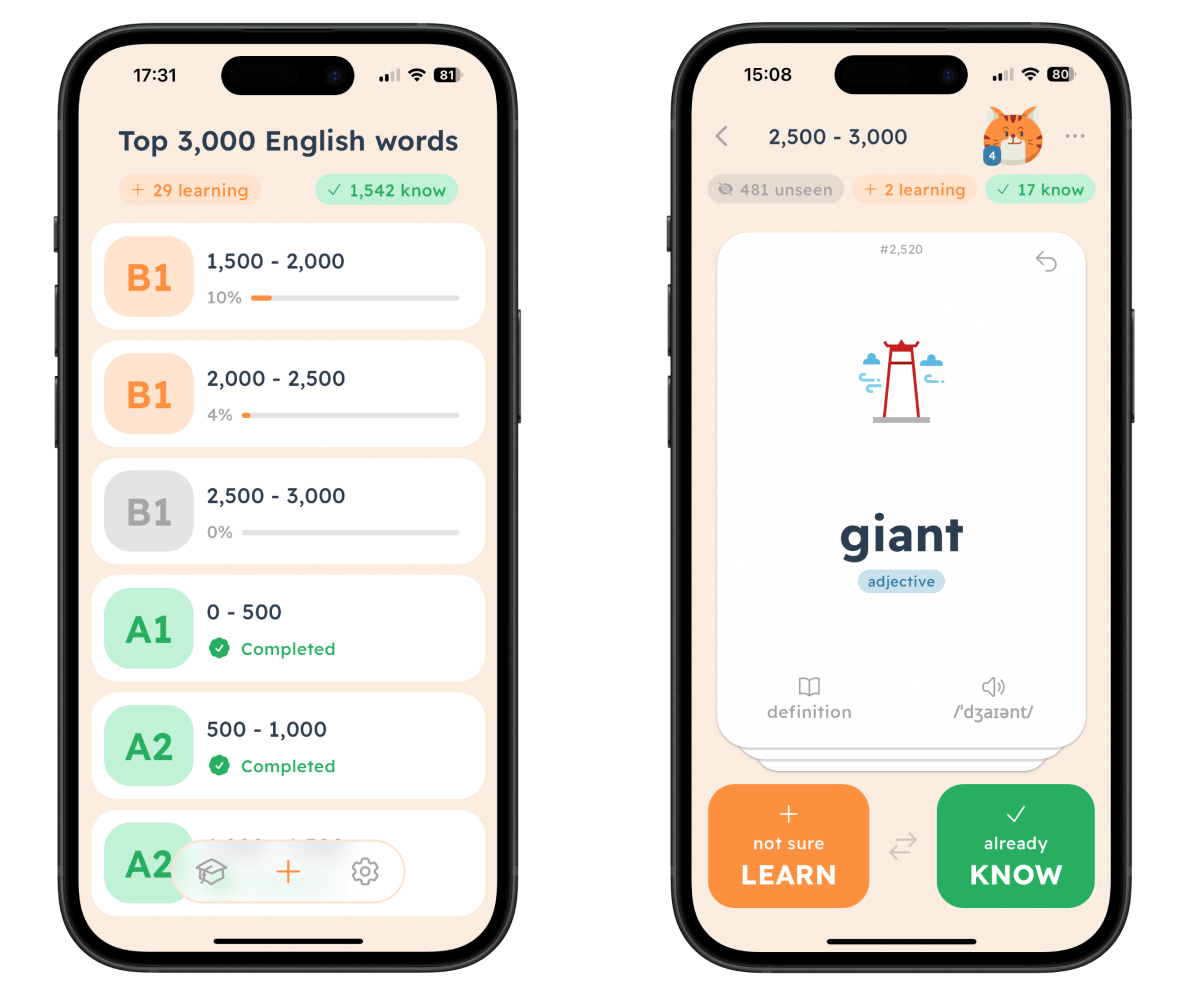
\includegraphics[width=0.8\textwidth]{src/figures/em-frequency-list.png}
    \caption{English Mind - Frequency List}
    \label{fig:em-frequency-list}
\end{figure}

\section{Active Recall and Flashcards}
\label{sec:em-active-recall}

Active recall is a learning method where students attempt to retrieve information without reference to the source material, contrasting with passive review where information is simply reread. Research from Washington University \cite{cite:rhkj2006_longterm_retention} demonstrates active recall's superiority for long-term retention: in a study of 120 students, active recall consistently outperformed passive review across various time intervals (5 minutes, 2 days, and 1 week), as shown in Figure \ref{fig:active-recall-passive-review-results}.

\begin{figure}[!h]
    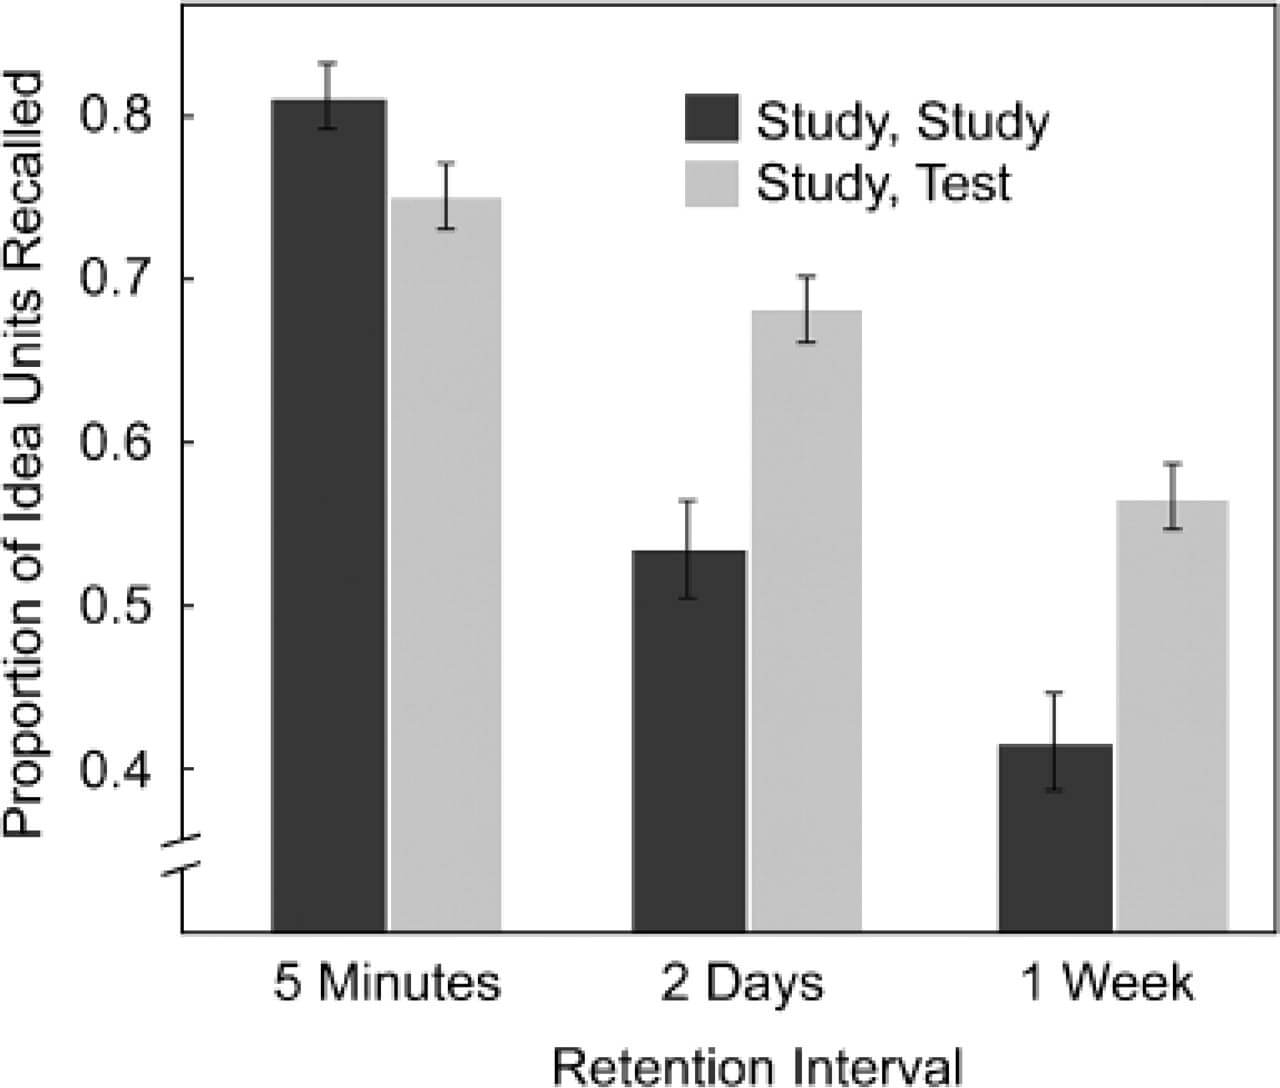
\includegraphics[width=0.7\textwidth]{src/figures/active-recall-passive-review-results.jpeg}
    \caption{Comparison of retention rates between active recall and passive review methods across different time intervals \cite{cite:rhkj2006_longterm_retention}}
    \label{fig:active-recall-passive-review-results}
\end{figure}

Flashcards represent a practical implementation of active recall, where information is split between two sides of a card, forcing active retrieval before verification.

English Mind implements flashcard-based active recall by presenting vocabulary words on the front and comprehensive word information (definition, usage examples, pronunciation, and native language translation) on the reverse, as shown in Figure \ref{fig:em-flashcards}. Users must attempt to recall the word's meaning before revealing the reverse side.

\begin{figure}[!h]
    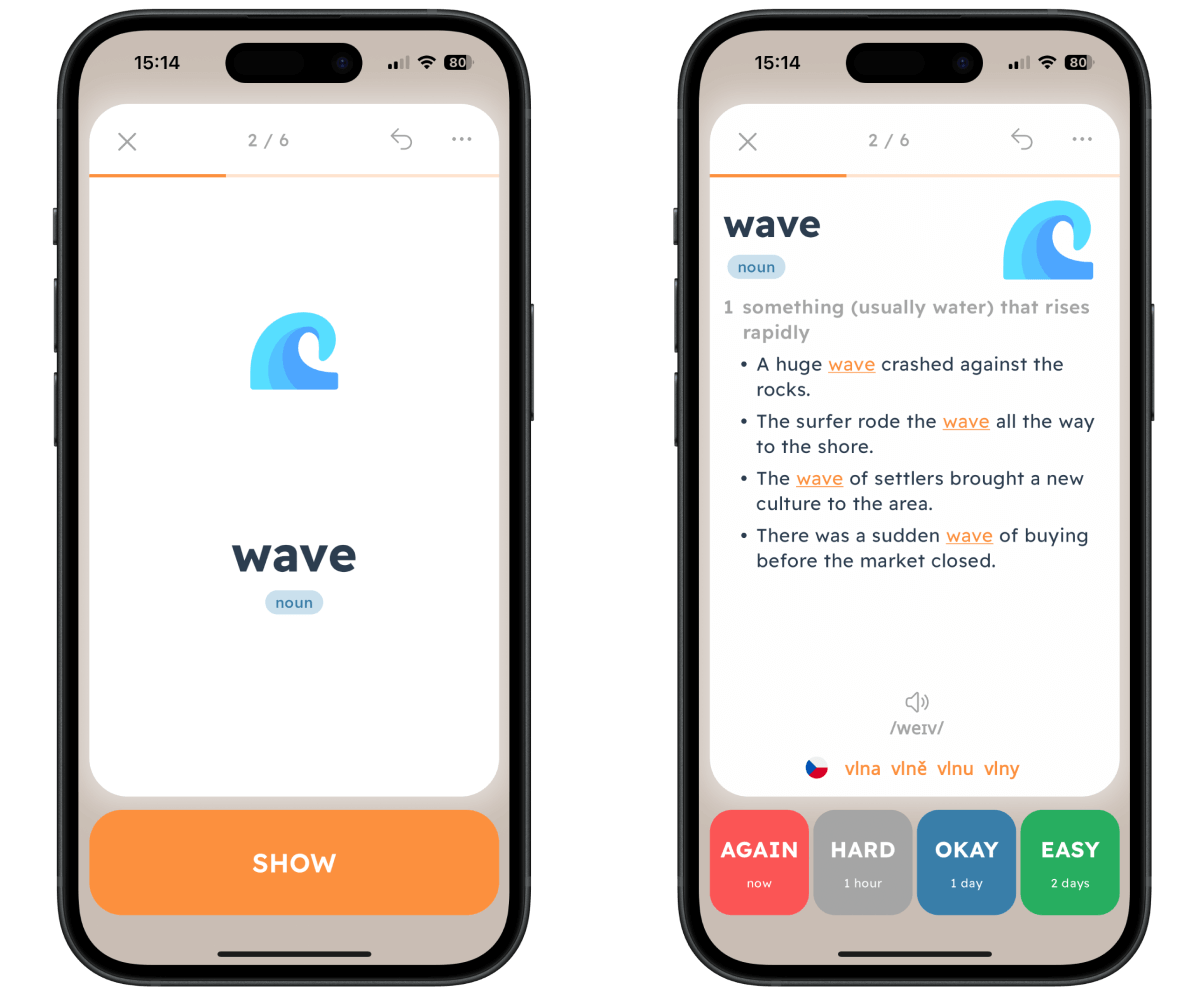
\includegraphics[width=0.9\textwidth]{src/figures/em-flashcards.png}
    \caption{English Mind - Active Recall Utilizing Flashcards}
    \label{fig:em-flashcards}
\end{figure}

\section{Spaced Repetition System (SRS)}

Spaced Repetition System (SRS) optimizes learning by adjusting intervals between review sessions based on recall performance. This method builds on Ebbinghaus's forgetting curve theory \cite{cite:ebbinghaus2013_memory_contribution_to_experimantal_psychology}, which demonstrates that information retention improves when review occurs just before predicted forgetting. Research shows that SRS increases learning efficiency by optimizing review timing and reducing unnecessary repetition \cite{cite:kang2016_spaced_repetiton_promotes_efficient_learning}.

The application implements SRS through a four-button feedback system (AGAIN, HARD, OKAY, EASY) that appears after each flashcard review, as shown in Figure \ref{fig:em-srs-flashcard}. Each button adjusts the next review interval: AGAIN and HARD decrease it, while OKAY and EASY increase it. Words consistently recalled over several months automatically transition from "LEARNING" to "KNOWN" status.

\begin{figure}[!h]
    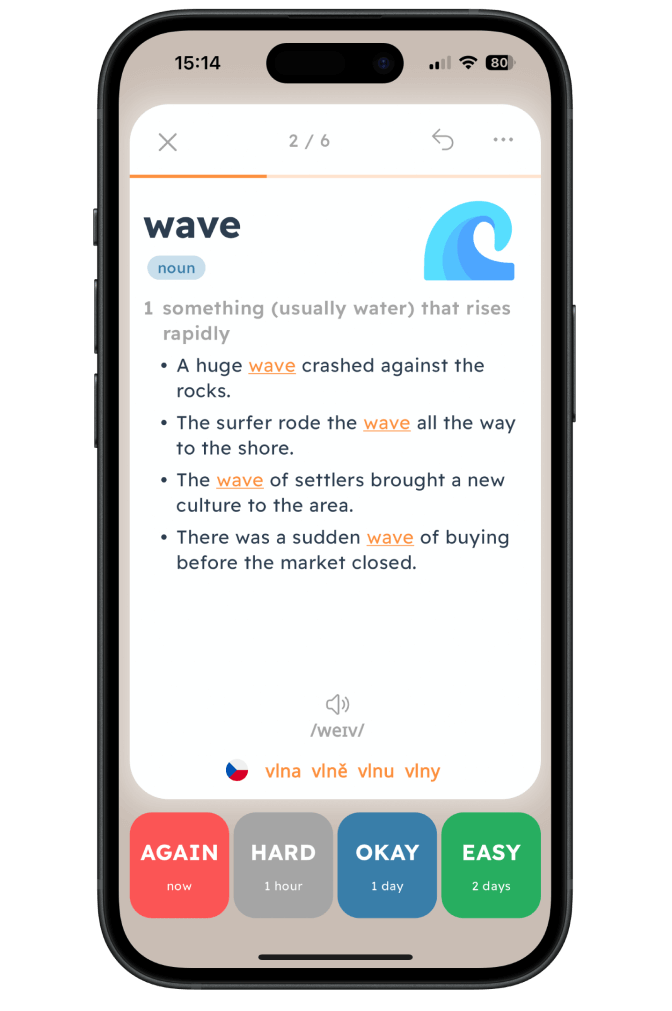
\includegraphics[width=0.6\textwidth]{src/figures/em-srs-flashcard.png}
    \caption{English Mind - SRS}
    \label{fig:em-srs-flashcard}
\end{figure}

\section{Application Workflow}

The application's learning process consists of two primary phases: vocabulary selection and practice. Figure \ref{fig:em-hta} illustrates the hierarchical breakdown of these tasks.

Users first browse the frequency-ordered vocabulary list, marking words as either "KNOWN" (already mastered) or "LEARNING" (to be studied). This initial classification ensures that learning efforts focus on appropriate vocabulary. Subsequently, words marked as "LEARNING" enter the practice phase, where they are studied through flashcards and systematically reviewed using spaced repetition.

\vspace{1cm}

\begin{figure}[!h]
    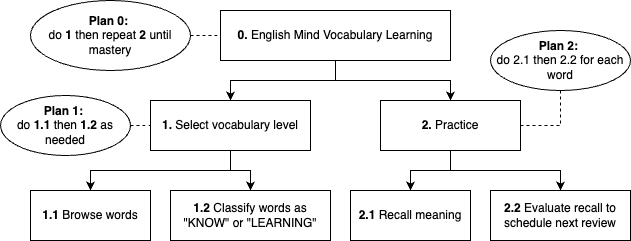
\includegraphics[width=1\textwidth]{src/figures/english_mind_workflow_THA.png}
    \caption{English Mind - Hierarchical Task Analysis of the core learning workflow}
    \label{fig:em-hta}
\end{figure}


\part{Analysis}
\chapter{Analysis of Gamification in Language Learning Applications}

Gamification is defined as "the use of game design elements in non-game contexts" \cite{cite:deterding2011_gamefulness}. In educational settings, it enhances learning activities through game mechanics to increase student engagement and motivation. The field encompasses numerous concepts, including streaks, achievements, leaderboards, progress tracking, social elements, virtual currencies, and much more \cite{cite:govender2021_gamification_elements_in_language_learning_apps}.

Traditional vocabulary learning methods often rely on mechanical repetition or passive reading, which can lead to decreased engagement and compromised learning outcomes. This challenge is particularly evident in language acquisition, where consistent practice is crucial for long-term retention. Gamification addresses these limitations by incorporating structured incentives for regular practice while maintaining learner engagement through various game mechanics.

While gamification offers numerous potential elements for implementation, this analysis focuses specifically on features that enhance vocabulary learning effectiveness. This chapter first examines the current gamification features in English Mind, identifying areas for potential enhancement. It then analyzes three prominent language learning applications — WordUp \cite{cite:wordup}, DuoCards \cite{cite:duocards}, and Duolingo \cite{cite:duolingo} — selected based on either their similarity to English Mind's learning approach or their innovative implementation of gamification elements. The chapter concludes with a comparative analysis of these applications and identifies key opportunities for improvement.\newpage

\section{English Mind}

English Mind currently implements minimal gamification features, consisting primarily of two basic progress visualization elements:

\begin{itemize}
    \item \textbf{Vocabulary Progress Overview} 
    \label{chap:em-progess-tracking}
    
    The application provides quantitative metrics of vocabulary acquisition progress, displaying the number of known words, words in active learning, and remaining words to be learned (see Figure \ref{fig:em-progress-tracking}). This statistical overview enables users to track their overall learning trajectory.

    \begin{figure}[!h]
        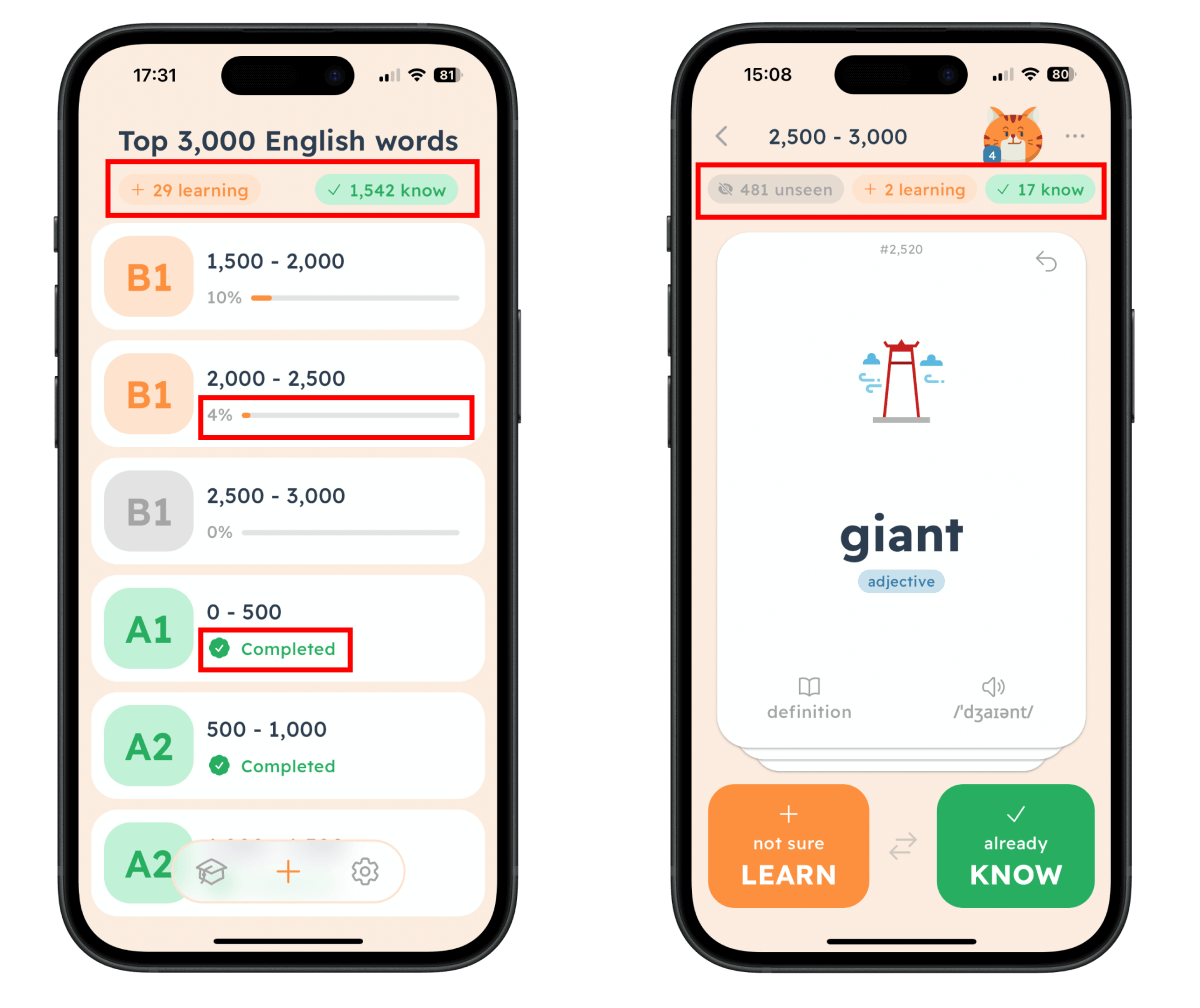
\includegraphics[width=0.9\textwidth]{src/figures/em-progress-tracking.png}
        \caption{English Mind - Vocabulary Progress Overview}
        \label{fig:em-progress-tracking}
    \end{figure}

    \item \textbf{Session Progress Indicator}
    
    A linear progress indicator during flashcard practice sessions provides visual feedback on session completion status. This basic implementation offers immediate context for session progress.
    
\end{itemize}

This limited implementation of gamification elements suggests significant potential for enhancement through more sophisticated engagement mechanisms, which will be examined through comparative analysis in subsequent sections.

\section{WordUp}

WordUp represents a particularly relevant case study as it shares the core learning methodologies with English Mind, combining frequency lists with spaced repetition and flashcard-based practice. With over 5 million downloads on Google Play \cite{cite:wordup_google_play}, its implementation of gamification elements provides comparative insights for potential enhancements to English Mind. The application implements three key gamification features:

\begin{itemize}
    \item \textbf{Diversified Flashcard Types}

    WordUp employs four variants of flashcards, each targeting different aspects of vocabulary acquisition (see Figure \ref{fig:wordup-flashcard-types}). This variation in exercise types helps maintain engagement while addressing multiple aspects of language acquisition — meaning comprehension, recall, spelling accuracy, and listening skills.
    
    \begin{itemize}
        \item Word-to-Definition matching
        \item Definition-to-Word recall
        \item Definition-to-Spelling association
        \item Audio-to-Spelling transcription
    \end{itemize}

    \begin{figure}[!h]
        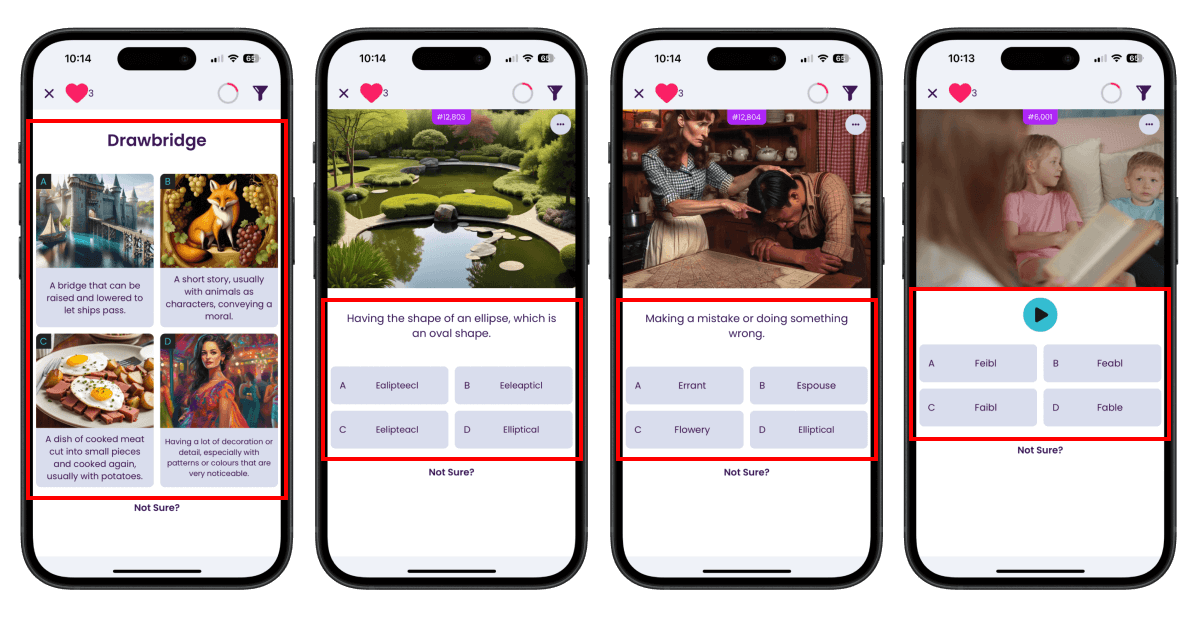
\includegraphics[width=1\textwidth]{src/figures/wordup-flashcard-types.png}
        \caption{WordUp - Flashcard Type Variations}
        \label{fig:wordup-flashcard-types}
    \end{figure}
    
    \item \textbf{Individual Word Progress Tracking}
    \label{sec:wordup-individual-word-progress-experience}
    
    The application implements a granular progress tracking system that visualizes individual word mastery through a numerical indicator (see Figure \ref{fig:wordup-word-progress}). This mechanism provides immediate feedback on learning progress at the word level.

    \begin{figure}[!h]
        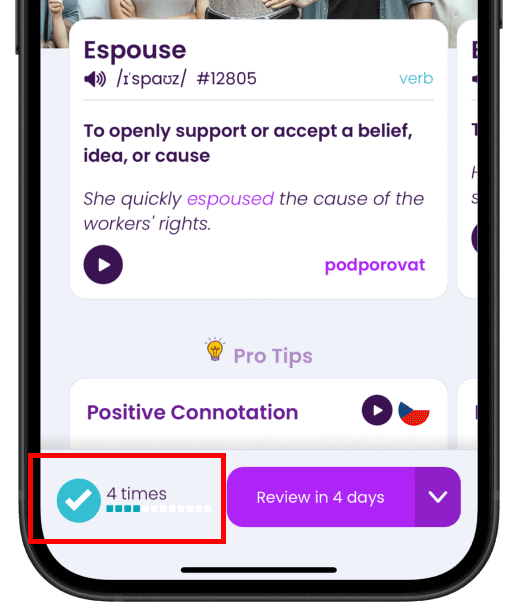
\includegraphics[width=0.35\textwidth]{src/figures/wordup-word-progress.png}
        \caption{WordUp - Individual Word Progress Indicator}
        \label{fig:wordup-word-progress}
    \end{figure}

    \item \textbf{Time-Based Goals and Social Competition}

    The application incorporates daily practice goals measured in minutes, complemented by a leaderboard system (see Figure \ref{fig:wordup-daily-goal}). This combination of personal goals and social comparison creates multiple motivation vectors for sustained engagement.

    \begin{figure}[!h]
        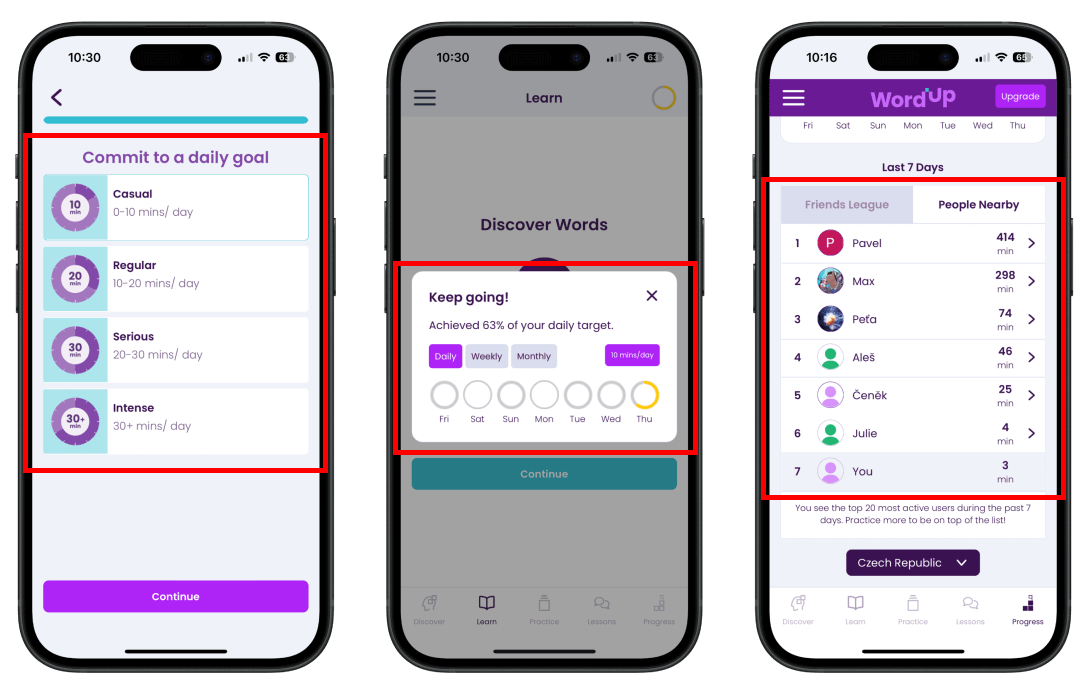
\includegraphics[width=0.99\textwidth]{src/figures/wordup-daily-goal.png}
        \caption{WordUp - Daily Goal and Leaderboard}
        \label{fig:wordup-daily-goal}
    \end{figure}

\end{itemize}

\section{DuoCards}

DuoCards, with over a million downloads on Google Play \cite{cite:duocards_google_play}, implements an SRS-based flashcard system for vocabulary acquisition. The application's gamification strategy centers on two primary mechanisms: diversified practice formats and an incentive-based progression system.

\begin{itemize}
    \item \textbf{Diversified Practice Formats}

    The application implements four distinct flashcard variants that systematically address different aspects of vocabulary acquisition (see Figure \ref{fig:duocards-flashcard-types}). This methodological variation facilitates comprehensive vocabulary acquisition while maintaining engagement through task diversity.

    \begin{itemize} 
         \item Bidirectional translation exercises
         \item Auditory comprehension and pronunciation exercises
         \item Multi-item matching exercises for vocabulary reinforcement
    \end{itemize}

    \begin{figure}[!h]
        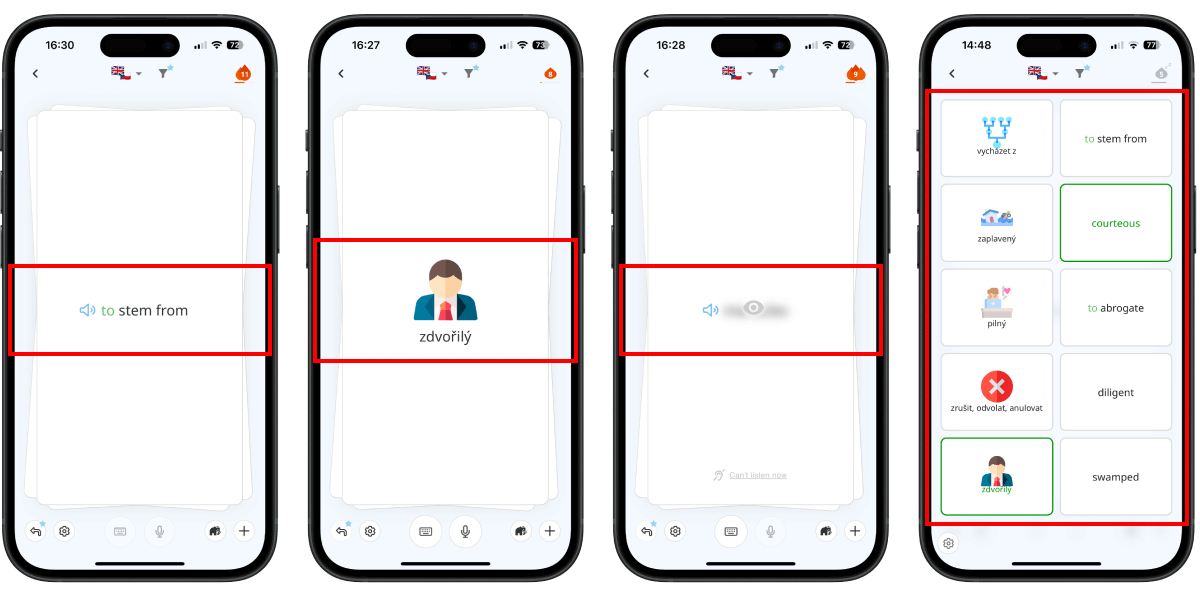
\includegraphics[width=0.98\textwidth]{src/figures/duocards-flashcard-types.png}
        \caption{DuoCards - Variation in Practice Formats}
        \label{fig:duocards-flashcard-types}
    \end{figure}
    
    \item \textbf{Virtual Currency and Achievement System}

    The application implements an experience-based reward system (XP) integrated with a customizable mascot interface (see Figure \ref{fig:duocards-memo}). This gamification mechanism creates a tangible reward structure where practice completion and vocabulary acquisition yield currency for environmental customization, thereby reinforcing consistent engagement patterns.

    \begin{figure}[!h]
        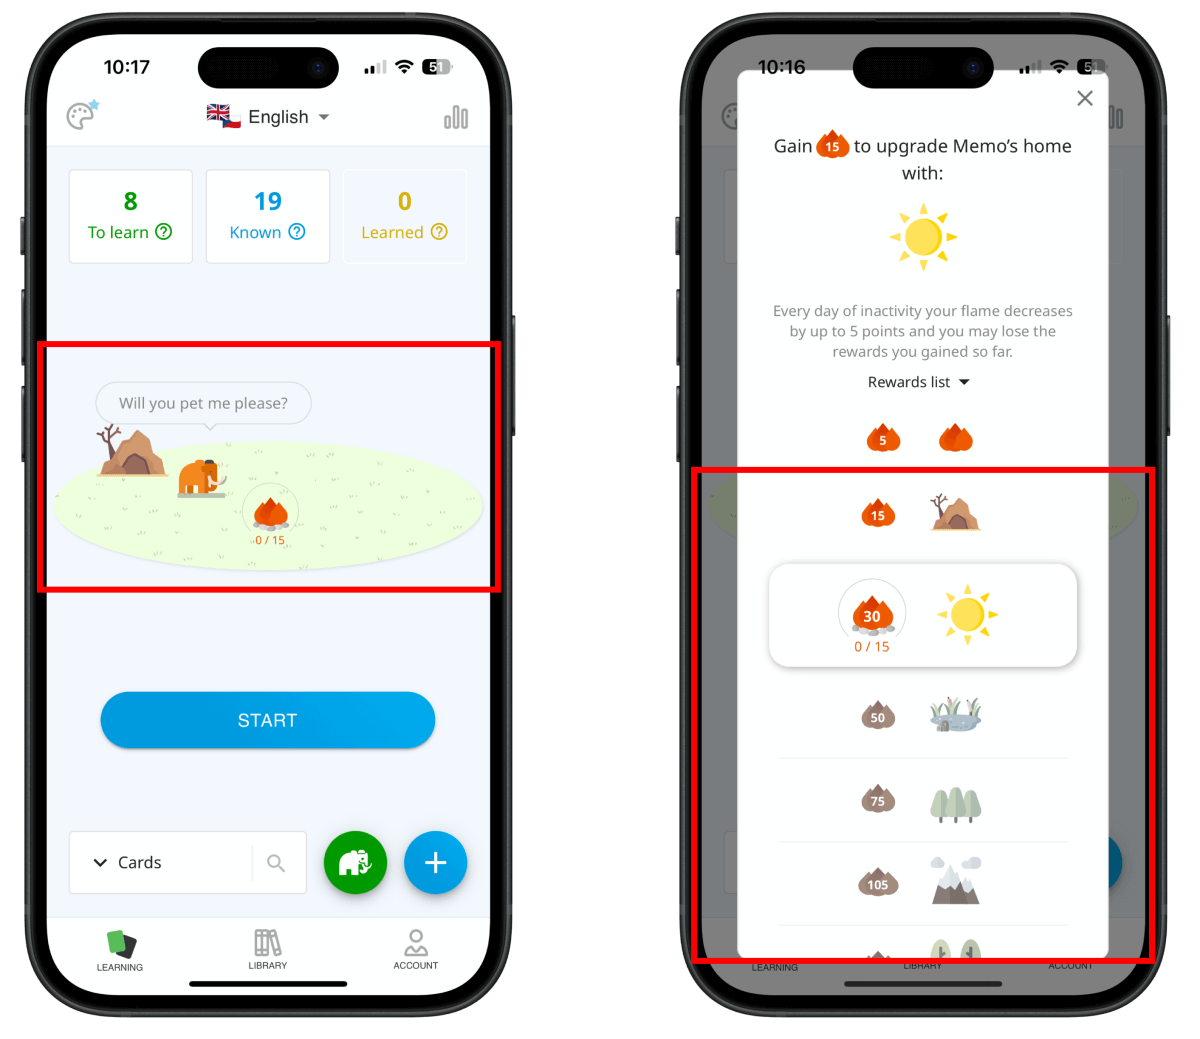
\includegraphics[width=0.7\textwidth]{src/figures/duocards-memo.png}
        \caption{DuoCards - Achievement-Based Customization}
        \label{fig:duocards-memo}
    \end{figure}

\end{itemize}

\section{Duolingo}

Duolingo, with over 100 million monthly active users \cite{cite:duolingo_2024q2}, has established significant precedent in digital language education gamification. While extensive research exists on Duolingo's comprehensive feature set, this analysis focuses on three key elements particularly relevant to English Mind's vocabulary learning context.

\begin{itemize}
    \item \textbf{Exercise Diversification}

    The application implements multiple exercise variants to reinforce vocabulary acquisition. This methodological variation addresses multiple aspects of language acquisition while maintaining engagement through task diversity (see Figure \ref{fig:duolingo-exercise-types}).

    \begin{itemize}
        \item Word-translation pair matching exercises
        \item Speech recognition-based pronunciation assessment
        \item Audio-to-text transcription for listening comprehension
    \end{itemize}

    \begin{figure}[!h]
        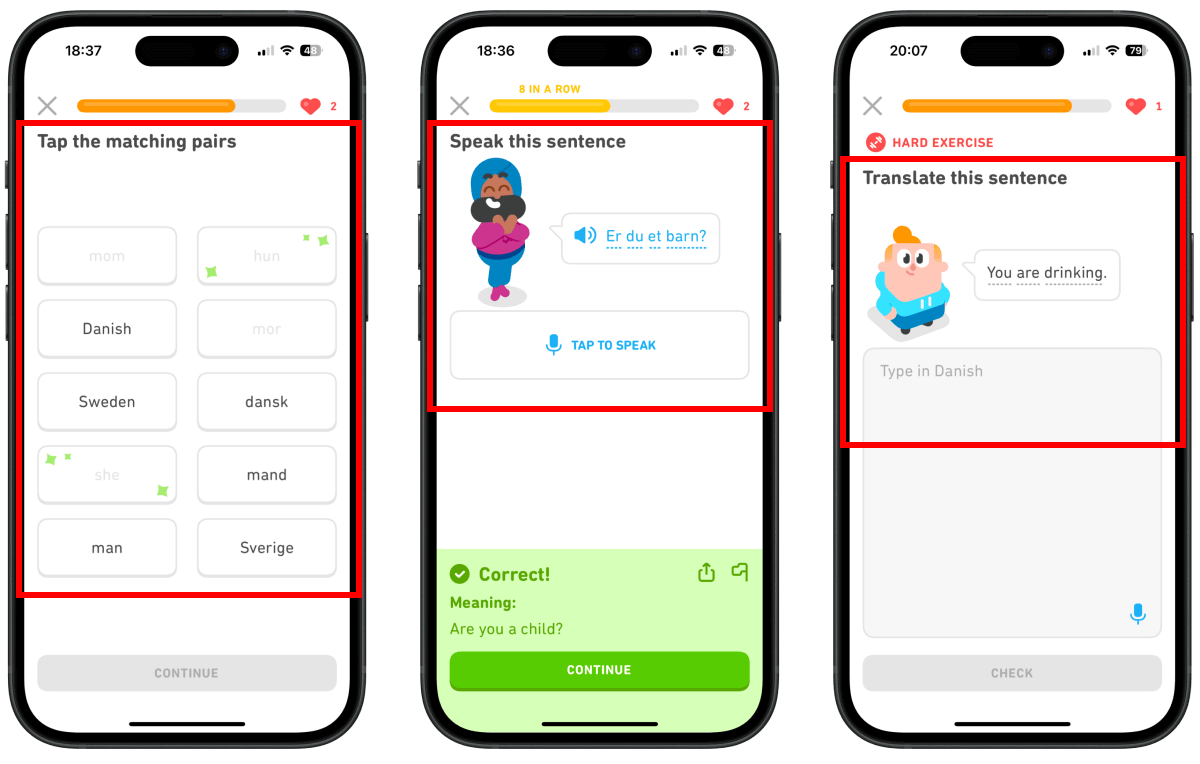
\includegraphics[width=0.9\textwidth]{src/figures/duolingo-exercise-types.png}
        \caption{Duolingo - Exercise Types}
        \label{fig:duolingo-exercise-types}
    \end{figure}
    \newpage
    \item \textbf{Post-Session Analytics}
    \label{sec:duolingo-lesson-review}

    The application provides immediate post-session feedback through quantitative metrics. This feedback mechanism facilitates progress tracking while reinforcing achievement through immediate performance visualization (see Figure \ref{fig:duolingo-lesson-review}).
    
    \begin{itemize}
        \item Performance accuracy
        \item Experience points acquired
        \item Time investment
        \item Streak metrics
    \end{itemize}

    \begin{figure}[!h]
        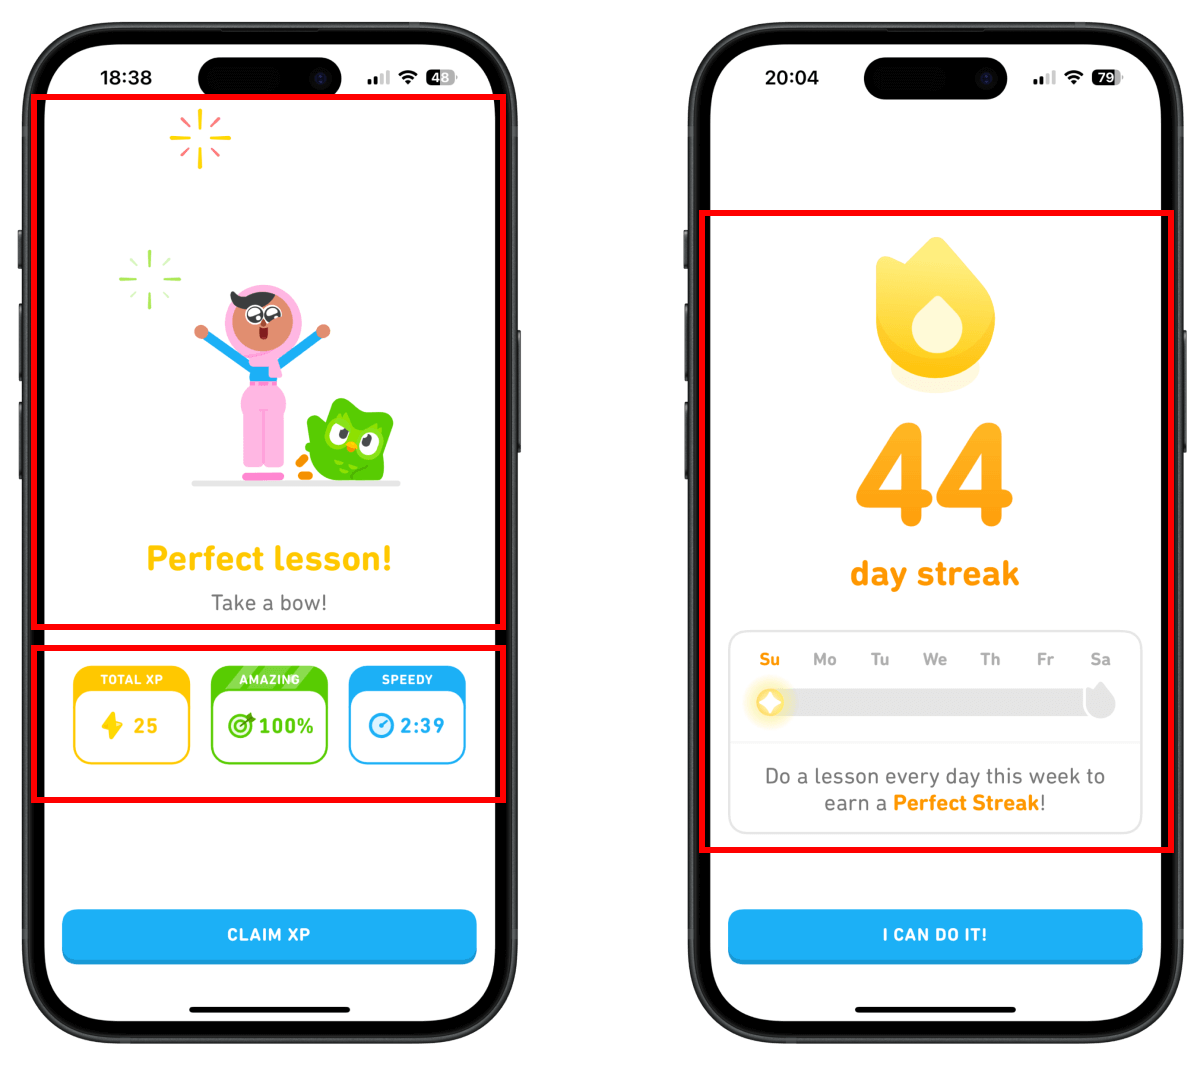
\includegraphics[width=0.8\textwidth]{src/figures/duolingo-lesson-review.png}
        \caption{Duolingo - Post-Session Analytics}
        \label{fig:duolingo-lesson-review}
    \end{figure}

    \item \textbf{Streak System}
    \label{sec:duolingo-streak-system}

    The application implements a streak-based tracking mechanism that incentivizes daily engagement. This system includes flexibility features ("Streak Freezes") to accommodate occasional missed sessions while maintaining motivation. The effectiveness is demonstrated by retention metrics, with 20\% of daily active users maintaining streaks exceeding one year \cite{cite:duolingo_2024q2}. The system is supported by a structured notification framework incorporating:
    
    \begin{itemize}
        \item Streak maintenance alerts
        \item Customizable practice reminders
        \item Achievement milestone recognition
    \end{itemize}

    \begin{figure}[!h]
        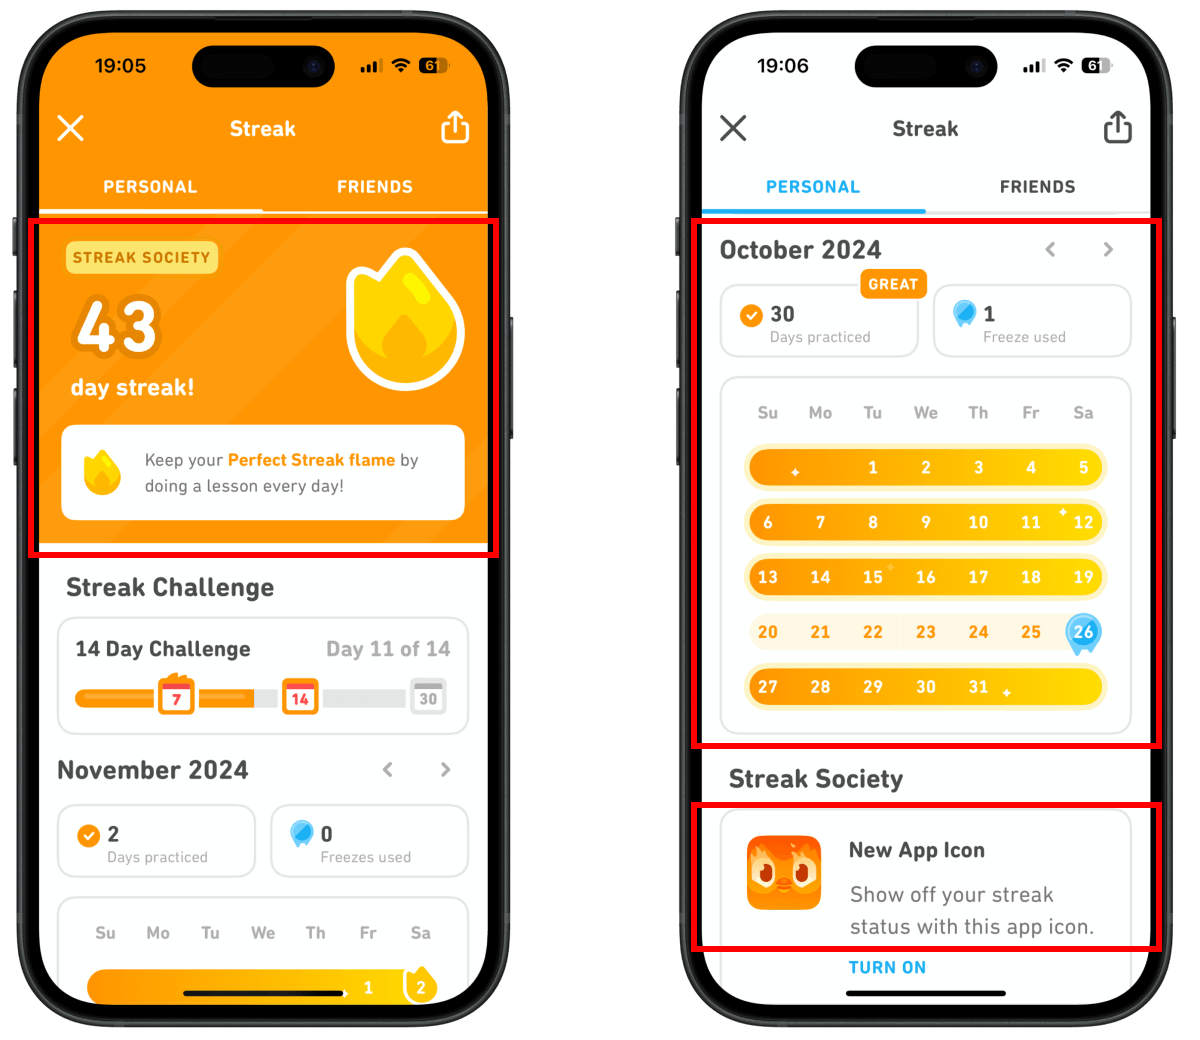
\includegraphics[width=0.8\textwidth]{src/figures/duolingo-streak.png}
        \caption{Duolingo - Streak System}
        \label{fig:duolingo-daily-streak}
    \end{figure}
\end{itemize}

\section{Comparison and Findings}

The comparative analysis of gamification features across the examined applications reveals distinct patterns in implementation approaches and feature adoption (Table \ref{tab:gamification-comparison}). The analysis yields three primary findings:
\begin{enumerate}
    \item Multiple exercise formats emerge as an industry standard, with WordUp, DuoCards, and Duolingo each implementing at least three distinct practice types. This contrasts with English Mind's single-format approach. The prevalence of varied exercise types suggests their effectiveness in both engagement and comprehensive vocabulary acquisition.

    \item Progress visualization implementations vary in granularity. While all applications provide aggregate progress metrics, WordUp's individual word progress tracking and Duolingo's post-session analytics demonstrate more sophisticated approaches to progress feedback.
    
    \item Engagement retention mechanisms vary across applications, with mainly Duolingo's streak system showing notable effectiveness.
\end{enumerate}


\begin{table}[h]
    \caption{Comparison of Gamification Features Across Applications}
    \label{tab:gamification-comparison}
    
    % Spacing between rows and columns
    \renewcommand{\arraystretch}{1.2}
    \setlength{\tabcolsep}{2pt}
    
    \begin{tabular}{l>{\centering}p{2cm}>{\centering}p{2cm}>{\centering}p{2cm}>{\centering\arraybackslash}p{2cm}}
        \toprule
        \textbf{Feature} & \textbf{English Mind} & \textbf{WordUp} & \textbf{DuoCards} & \textbf{Duolingo} \\
        \midrule
        \multicolumn{5}{l}{\textbf{Flashcard Variations}} \\
        Multiple flashcard types & \textemdash & \ding{51} & \ding{51} & \ding{51} \\
        Spelling exercises & \textemdash & \ding{51} & \ding{51} & \ding{51} \\
        Matching exercises & \textemdash & \ding{51} & \ding{51} & \ding{51} \\
        Speaking exercises & \textemdash & \textemdash & \textemdash & \ding{51} \\
        \midrule
        \multicolumn{5}{l}{\textbf{Progress Tracking}} \\
        Overall progress visualization & \ding{51} & \ding{51} & \ding{51} & \ding{51} \\
        Practice session progress bar & \ding{51} & \ding{51} & \ding{51} & \ding{51} \\
        Individual word progress & \textemdash & \ding{51} & \textemdash & \textemdash \\
        \midrule
        \multicolumn{5}{l}{\textbf{Streaks and Daily Goals}} \\
        Streak system & \textemdash & \textemdash & \ding{51} & \ding{51} \\
        Daily word goal & \ding{51} & \textemdash & \textemdash & \textemdash \\
        Daily time goal & \textemdash & \ding{51} & \textemdash & \textemdash \\
        \midrule
        \multicolumn{5}{l}{\textbf{Rewards and Motivation}} \\
        Virtual currency & \textemdash & \textemdash & \ding{51} & \ding{51} \\
        Post-practice review & \textemdash & \textemdash & \textemdash & \ding{51} \\ 
        Leaderboards & \textemdash & \ding{51} & \textemdash & \ding{51} \\
        Mascot upgrade system & \textemdash & \textemdash & \ding{51} & \textemdash \\
        \bottomrule
    \end{tabular}
\end{table}
\chapter{Selected Gamification Features for English Mind}

Based on the analysis of existing applications and their gamification features, we have identified several opportunities to enhance the English Mind application. Our selection process focused on features that meet three key criteria:

\begin{enumerate}
    \item \textbf{High Impact Potential:} Features that have demonstrated effectiveness in other applications and show potential for improving user engagement and learning outcomes.
    
    \item \textbf{Alignment with Core Concepts:} Features that complement and enhance English Mind's fundamental learning principles of frequency-based vocabulary acquisition and spaced repetition.
    
    \item \textbf{Implementation Feasibility:} Solutions that can be realistically implemented within the existing application architecture and technical constraints.
\end{enumerate}

Rather than attempting to implement every possible gamification feature, we have prioritized a focused set of enhancements that we believe will provide the most significant benefits to users. For each proposed feature, we have developed detailed high-fidelity prototypes and implementation considerations. These designs demonstrate how each gamification element will be integrated into the existing application while maintaining its core educational value. These proposed features have been organized into two main categories:

\begin{itemize}
    \item \textbf{Category 1: Enhanced Practice Experience}
    
    Improvements to the core flashcard practice system to make it more engaging and effective (see Section \ref{sec:em-gamification-practice-experience}).
    
    \item \textbf{Category 2: Consistent Practice Motivation}
    
    Features designed to encourage regular app usage and maintain long-term user engagement (see Section \ref{sec:em-gamification-practice-motivation}).
\end{itemize}

\section{Category 1: Enhanced Practice Experience}
\label{sec:em-gamification-practice-experience}
The core flashcard practice experience is fundamental to English Mind's learning methodology. While the current implementation is functional, our analysis revealed several opportunities to make it more engaging and effective through gamification. This section presents three key enhancements to the practice experience, each designed to increase user engagement while maintaining the app's educational integrity.

\subsection{Diversified Flashcard Types}

The current English Mind flashcard system uses a single format where users view an English word and recall its meaning. While effective, our analysis of similar applications revealed that incorporating multiple flashcard types can enhance engagement and address different aspects of vocabulary acquisition. We propose expanding the system to include five distinct flashcard types, each targeting specific learning objectives (see Figure \ref{fig:em-prototype-flashcard-types}).

\begin{itemize}
    \item \textbf{Basic Meaning Recognition (Existing)}

    The current format where users see an English word and recall its meaning will be maintained as the foundation of the practice system. This format effectively tests basic word recognition and meaning recall (see Section \ref{sec:em-active-recall-flashcards}).

    \item \textbf{Word Matching (Two Variants)}
    
    Following the successful implementation in applications like Duolingo and WordUp, we propose two matching exercise variants:
    
    \begin{itemize}
        \item \textbf{Word-Translation Matching:} Users match English words with their corresponding translations, presented in sets of five pairs.
        
        \item \textbf{Word-Definition Matching:} Similar to the translation variant, but users match English words with their definitions, reinforcing deeper understanding of word meanings.
    \end{itemize}

    \item \textbf{Word Spelling}
    
    This exercise type presents users with a word's definition and a contextual sentence containing a blank space. Users must correctly spell the target word to complete the sentence. To assist learning, an audio pronunciation button is available. The system evaluates spelling accuracy and provides immediate feedback.
    \newpage

    \item \textbf{Word Pronunciation}

    Users are shown an English word and prompted to pronounce it correctly. The flashcard displays both the word and its IPA (International Phonetic Alphabet) transcription. The system evaluates pronunciation accuracy using speech recognition technology, providing binary feedback (correct/incorrect). Understanding that not all practice environments are suitable for speaking exercises, users can opt to skip these cards when needed.

\end{itemize}

\begin{figure}[!h]
    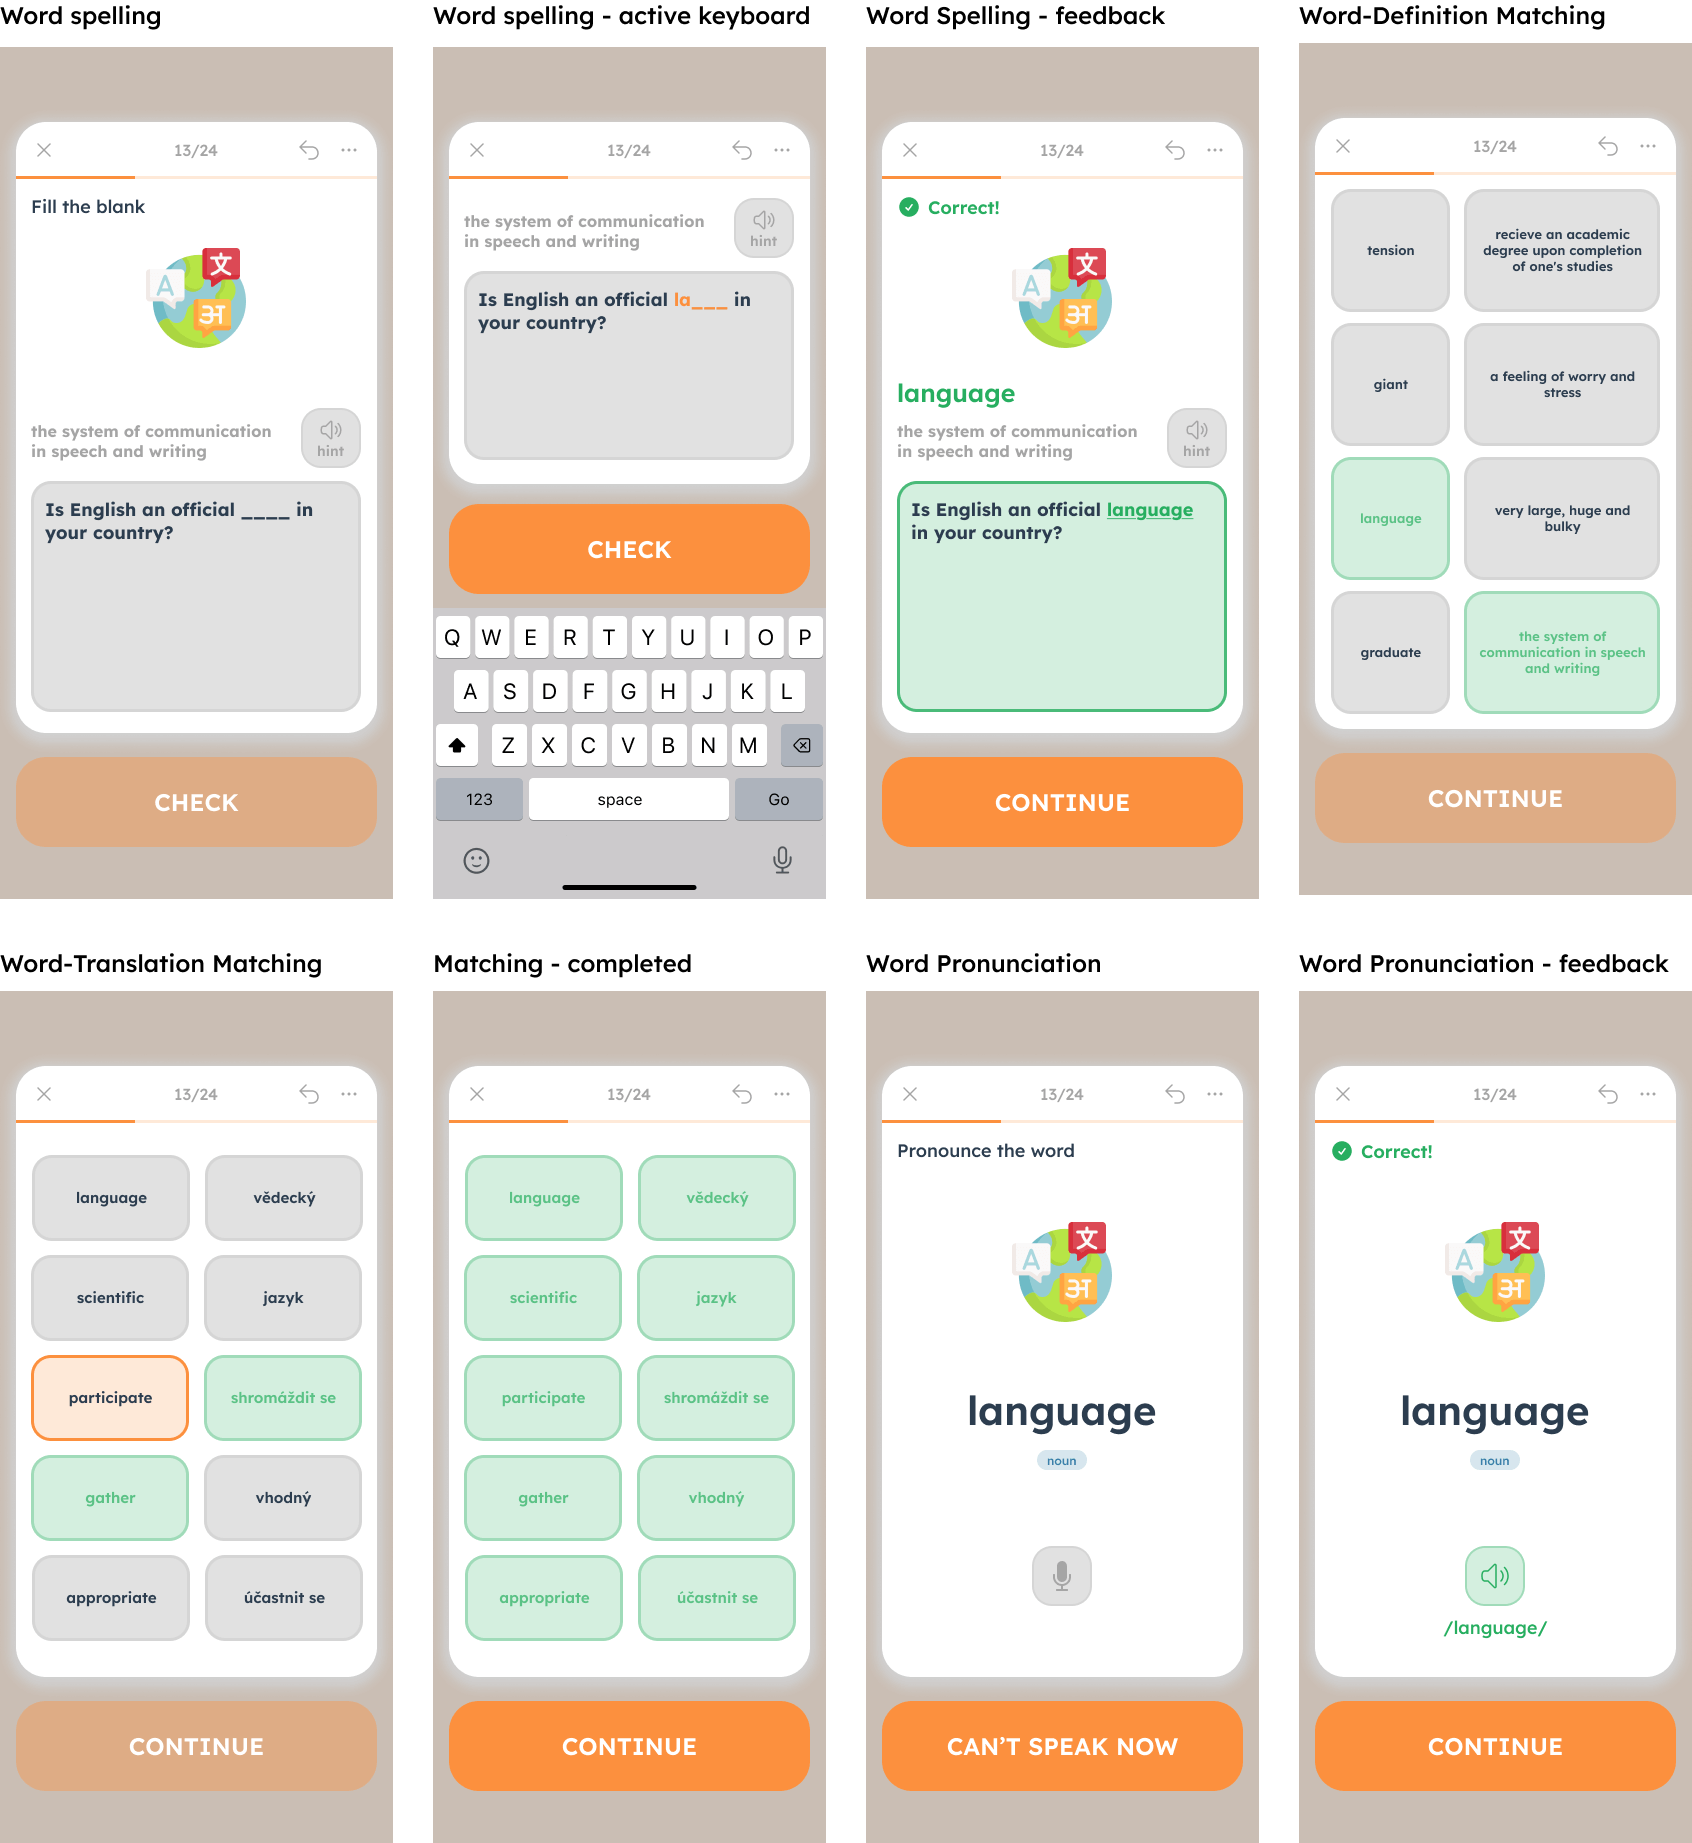
\includegraphics[width=1\textwidth]{src/figures/em-prototype-flashcards.png}
    \caption{English Mind - Prototype: Flashcard Types}
    \label{fig:em-prototype-flashcard-types}
\end{figure}

\subsubsection{Implementation Considerations}

The integration of new flashcard types requires careful consideration of both the spaced repetition system and the distribution of different card types during practice sessions.

To maintain the integrity of the existing spaced repetition system, only the basic meaning recognition flashcards will carry spaced repetition metadata and influence the scheduling of words. The additional flashcard types will serve as supplementary practice exercises without affecting the core SRS algorithm. This approach ensures the proven effectiveness of the current SRS remains unchanged, while additional practice types enhance learning without disrupting the established review schedule. Furthermore, this design allows user progress tracking to remain clear and consistent throughout the learning process.

The distribution of flashcard types within a practice session follows a structured approach that ensures varied practice while maintaining focus on core vocabulary acquisition through the primary flashcard type:

\begin{itemize}
    \item \textbf{Primary Flashcards:} Basic meaning recognition flashcards appear first in the daily queue, maintaining their role as the foundation of the spaced repetition learning system.
    
    \item \textbf{Supplementary Flashcards:} After completing the primary flashcards, users encounter the following types in randomized order:
    \begin{itemize}
        \item \textbf{Matching Flashcards:} Appear once for every five words in practice, grouping words into logical sets
        \item \textbf{Spelling Flashcards:} Randomly distributed throughout the supplementary practice
        \item \textbf{Pronunciation Flashcards:} Limited to newly introduced words and appear less frequently than other types
    \end{itemize}
\end{itemize}

\subsubsection{Expected Impact}

The diversification of flashcard types is expected to yield several benefits:

\begin{itemize}
    \item \textbf{Enhanced Engagement:} Variety in flashcard types reduces monotony and maintains user interest throughout longer practice sessions.
    
    \item \textbf{Comprehensive Learning and Retention:} Encountering words through diverse flashcard types (recognition, matching, spelling, and pronunciation) creates multiple memory pathways, leading to stronger and longer-lasting vocabulary mastery.
    
\end{itemize}

\subsection{Individual Word Progress Tracking}

Building upon the success of WordUp's individual word progress tracking (see Section \ref{sec:wordup-individual-word-progress-experience}), we propose implementing a visual progress indicator system that integrates seamlessly with English Mind's existing spaced repetition system. This feature provides users with clear, immediate feedback on their progress with each vocabulary item, helping them understand where they stand in the learning journey for specific words.

\subsubsection{Five-Stage Progress System}

The visual indicator system maps the existing spaced repetition intervals into five distinct stages. This system serves purely as a user-friendly representation of progress and does not modify the underlying SRS algorithm:


\begin{itemize}
    \item \textbf{Starting (Stage 1)}
    
    Represents words in their first 24 hours after introduction. These words are in the early stages of learning and require frequent review to establish basic recognition.
    
    \item \textbf{Familiarizing (Stage 2)}
    
    Covers words practiced between 1 day and 1 week. During this stage, words still require frequent reviews to build early recall strength and establish memory patterns.
    
    \item \textbf{Reinforcing (Stage 3)}
    
    Includes words with review intervals of 1-3 weeks. At this stage, users can recall words reliably, demonstrating consistent retention with moderate repetition intervals.
    
    \item \textbf{Strengthening (Stage 4)}
    
    Represents words practiced at 3-week to 3-month intervals. Users show strong confidence in recall, requiring significantly less frequent review as the word becomes well-established in long-term memory.
    
    \item \textbf{Almost Mastered (Stage 5)}
    
    Indicates words that have reached intervals of 3-8 months between reviews. These words are approaching full mastery, requiring only rare reviews to maintain retention. Once a word exceeds the 8-month interval, it will be marked as "known" and graduate from the regular review system.
\end{itemize}

\subsubsection{Visual Implementation}

The progress indicator appears in the top-left corner of primary flashcards (see Figure \ref{fig:em-prototype-word-progress}). It consists of five sequential boxes that fill progressively as the word advances through the stages, providing an intuitive visualization of progress. This design choice ensures the indicator is visible but not distracting from the primary learning task.

\begin{figure}[!h]
    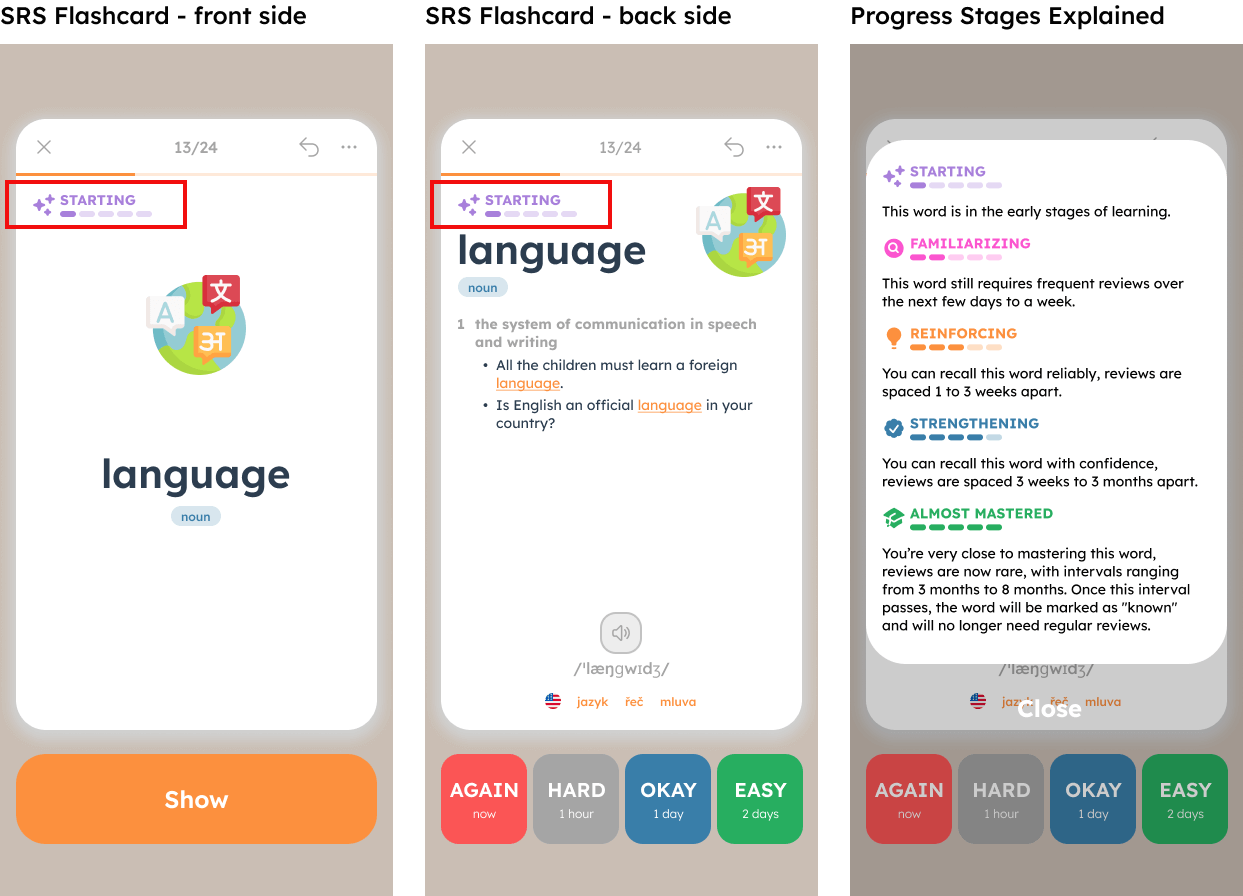
\includegraphics[width=1\textwidth]{src/figures/em-prototype-progress-system.png}
    \caption{English Mind - Prototype: Individual Word Progress Indicator (highlighted in red)}
    \label{fig:em-prototype-word-progress}
\end{figure}

\subsubsection{Integration with Existing SRS}

The progress tracking system is designed to work in harmony with the existing spaced repetition algorithm. Progress stages are determined automatically based on the word's current interval in the SRS system, with stages advancing or regressing according to review performance. This implementation leverages existing SRS metadata, requiring minimal additional computational overhead.

\subsubsection{Expected Impact}

The implementation of individual word progress tracking is expected to provide several benefits:

\begin{itemize}
    \item \textbf{Enhanced Motivation and Engagement:} Visual progress indicators create a game-like element that provides a sense of achievement as words advance through different stages.
    
    \item \textbf{Simplified Learning Metrics:} The staged system provides tangible feedback on the learning journey, making abstract concepts like spaced repetition more concrete and understandable.
\end{itemize}

\subsection{Post-Practice Review}

Drawing inspiration from Duolingo's successful implementation of post-practice feedback (see Section \ref{sec:duolingo-lesson-review}), we propose adding an engaging post-practice summary screen to English Mind. This feature provides immediate feedback and reinforcement after completing a practice session, helping users track their progress and maintain motivation.

\subsubsection{Post-Practice Review Screen Components}

The post-practice review screen consists of several key elements (see Figure \ref{fig:em-prototype-practice-review}):

\begin{itemize}
    \item \textbf{Practice Statistics}
    
    Clear visualization of practice session metrics including the number of words practiced and time spent practicing.
    
    \item \textbf{Mascot Interaction}
    
    The app's mascot appears with randomly selected poses to add personality to the user experience.
    
    \item \textbf{Motivational Messages}
    
    A rotating collection of encouraging messages that vary based on factors such as the number of words practiced, time spent practicing, and time of day.
    
    \item \textbf{Celebratory Animation}
    
    A confetti animation plays when the review screen appears, providing immediate positive reinforcement for completing the practice session. The animation is optimized to ensure smooth and lightweight performance across different devices.
\end{itemize}

\begin{figure}[!h]
    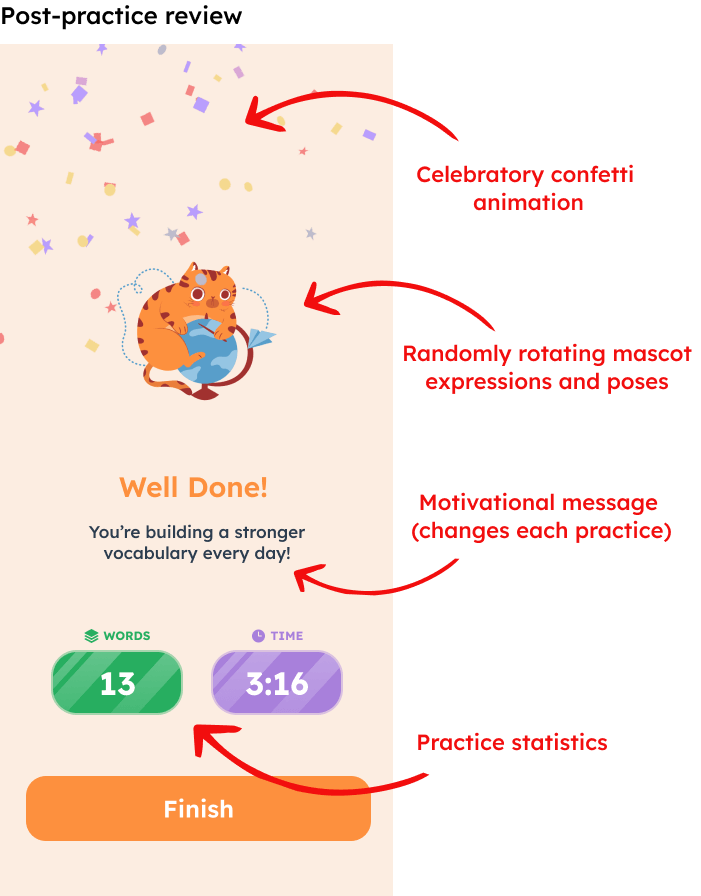
\includegraphics[width=0.8\textwidth]{src/figures/em-prototype-review.png}
    \caption{English Mind - Prototype: Post-Practice Review Screen}
    \label{fig:em-prototype-practice-review}
\end{figure}

\subsubsection{Expected Impact}

The implementation of a post-practice review screen is expected to:

\begin{itemize}
    \item \textbf{Increase Practice Completion:} The anticipation of positive feedback and celebration may motivate users to complete their practice sessions.
    
    \item \textbf{Boost User Satisfaction:} Immediate positive reinforcement through animations and encouraging messages creates a more rewarding experience.
\end{itemize}

\newpage

\section{Category 2: Consistent Practice Motivation}
\label{sec:em-gamification-practice-motivation}

Regular practice is crucial for effective vocabulary acquisition and retention. Currently, English Mind lacks features that promote consistent engagement, so we propose implementing a streak system — a feature that has proven highly effective in Duolingo's learning ecosystem (see Section \ref{sec:duolingo-streak-system}).

\subsection{Streak System}

The streak system is built on the fundamental requirement of learning at least one new word each day to maintain an active streak. Users must mark at least one word as "learning" each day and then review it at their daily queue of flashcards.This requirement ensures meaningful progress while keeping the daily commitment manageable for users. 

To support the effectiveness of the spaced repetition system, new words are strategically placed at the end of the review queue. This placement naturally encourages users to complete their due reviews before accessing the newly added words.

The system intentionally adopts a simplified approach, omitting streak features like "freeze" or streak recovery options. This deliberate choice allows us to establish and validate the core streak mechanics first, while features like streak freezes could be introduced in future iterations based on user feedback and engagement patterns.

\subsubsection{Visual Implementation}

The streak counter is prominently displayed at the top of the main screen (see Figure \ref{fig:em-prototype-streak}). This implementation includes a clear numerical display of consecutive practice days, with visual states that reflect the streak's status: a bright, golden appearance for active streaks, and a faded, shadowed appearance when the streak is at risk of being lost.

Upon completing the daily flashcard practice and increasing the streak, a celebration screen appears to reinforce the user's achievement (see Figure \ref{fig:em-prototype-streak}). This screen showcases the updated streak count alongside a weekly progress view displaying the current week's streak activity (Monday through Sunday). When users maintain a perfect week of daily practice, these seven days are highlighted within a special golden frame, providing additional visual recognition for consistent engagement.

\newpage

\begin{figure}[!h]
    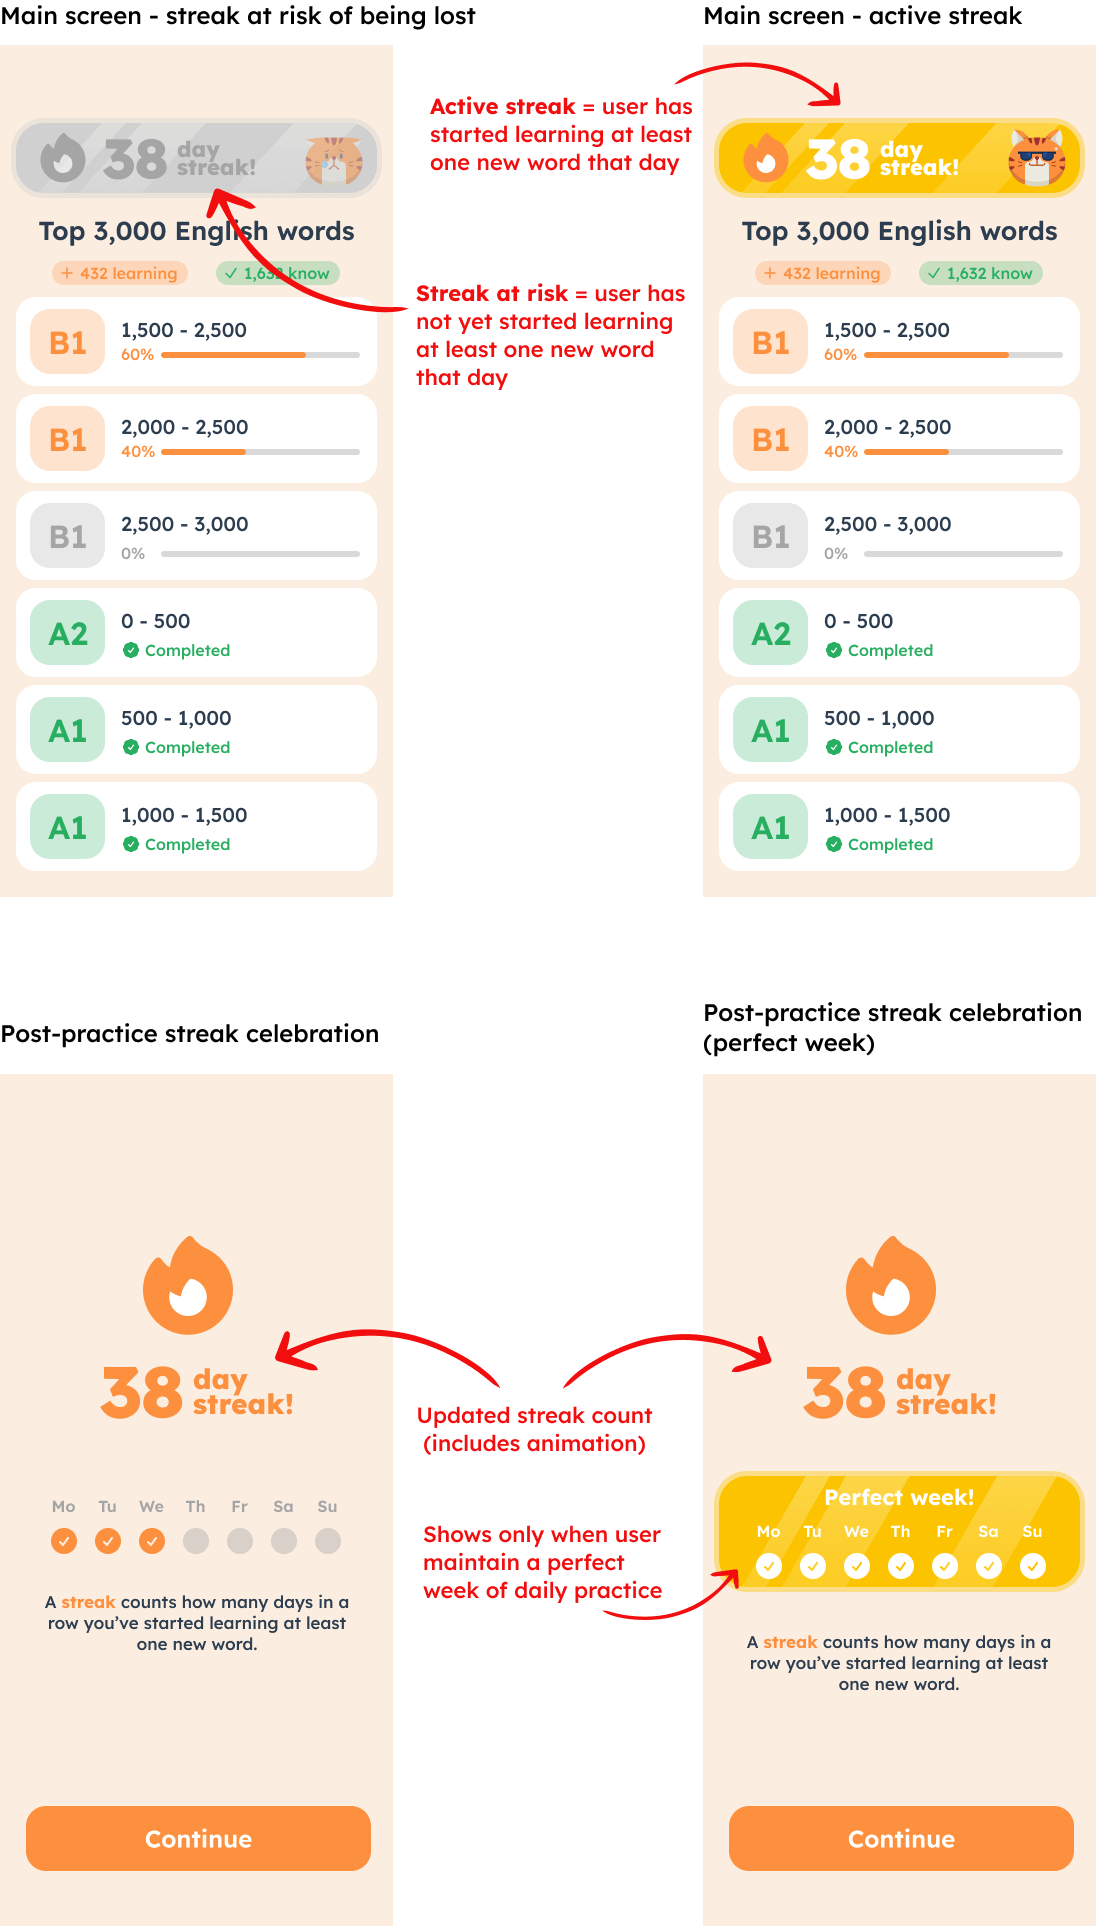
\includegraphics[width=0.9\textwidth]{src/figures/em-prototype-streak.png}
    \caption{English Mind - Prototype: Streak Implementation}
    \label{fig:em-prototype-streak}
\end{figure}

\subsubsection{Expected Impact}

The streak system is designed to serve multiple pedagogical and motivational purposes:

\begin{itemize}
    \item \textbf{Establish Daily Practice Habits:} By providing a clear, visible metric for consistency, it helps users establish and maintain daily practice habits.
    
    \item \textbf{Encourage Complete Reviews:} The strategic placement of new words after due flashcards naturally encourages users to complete their spaced repetition queue.
\end{itemize}

\chapter{User Testing}

This chapter describes the methodology and results of user testing conducted on the previously proposed and designed gamification features for English Mind. The testing focused on evaluating the clarity, intuitiveness, and potential effectiveness of the new gamification elements.

\section{Testing Methodology}

Two distinct user groups were selected for testing to provide diverse perspectives. Group A consisted of participants with prior experience using language learning applications, while Group B included participants without significant experience in this area.

\begin{itemize}
    \item \textbf{Group A (Experienced Users):}
    \begin{itemize}
        \item 6 participants aged 18-45
        \item Regular users of apps like Duolingo, WordUp, or Duocards
        \item Familiar with gamification concepts through regular usage of language learning applications (even without knowing the formal terminology)
    \end{itemize}

    \item \textbf{Group B (Novice Users):}
    \begin{itemize}
        \item 6 participants aged 18-45
        \item Interest in learning English vocabulary
        \item Limited exposure to language learning applications
    \end{itemize}
\end{itemize}

The testing was conducted in a controlled, quiet environment where participants interacted with high-fidelity interactive prototypes on mobile devices. Each session lasted between 30-45 minutes and was documented through screen and audio recordings.

Data collection during the testing sessions combined several methods to gather comprehensive feedback about the gamification features. Participants were encouraged to think aloud while interacting with the prototype, sharing their thoughts and reactions to different elements. This verbal feedback was supplemented by observation notes documenting user behavior, particularly noting any points of confusion or excitement. After completing the test scenario (see Section \ref{sec:test-scenario}), participants filled out a structured questionnaire rating various aspects of the gamification features on a 5-point Likert scale (see Table \ref{tab:questionnaire}). The questionnaire focused on key metrics such as feature clarity, perceived usefulness, and likelihood of maintaining engagement.


\begin{table}[h]
    \centering
    \caption{User Testing Questionnaire}
    \label{tab:questionnaire}
    \makebox[\textwidth][c]{
        \begin{tabular}{|p{0.9\textwidth}|c|c|c|c|c|}
            \hline
            \multicolumn{6}{|l|}{\small 1 = Strongly Disagree, 2 = Disagree, 3 = Neutral, 4 = Agree, 5 = Strongly Agree} \\
            \hline
            \textbf{Question} & \textbf{1} & \textbf{2} & \textbf{3} & \textbf{4} & \textbf{5} \\
            \hline
            \multicolumn{6}{|l|}{\textbf{Practice Flashcards Experience}} \\
            \hline
            1. The different types of flashcards made practice more engaging & & & & & \\
            \hline
            2. Each flashcard type's instructions were clear and easy to understand & & & & & \\
            \hline
            3. The variety in flashcard types helped me learn vocabulary more effectively & & & & & \\
            \hline
            4. The distribution of different flashcard types felt well-balanced & & & & & \\
            \hline
            5. The five-stage individual word progress indicator was easy to understand & & & & & \\
            \hline
            6. Seeing my progress for individual words motivated me to practice more & & & & & \\
            \hline
            7. The individual word progress indicator's placement was visually clear without being distracting & & & & & \\
            \hline
            8. I found the progress tracking helpful for understanding my learning journey & & & & & \\
            \hline
            9. The practice statistics provided useful information about my session & & & & & \\
            \hline
            10. The celebratory animations made completing practice more rewarding & & & & & \\
            \hline
            11. The review screen motivated me to complete future practice sessions & & & & & \\
            \hline
            \multicolumn{6}{|l|}{\textbf{Streak System}} \\
            \hline
            12. The streak system's requirements were clear and easy to understand & & & & & \\
            \hline
            13. The visual states (active/at risk) effectively communicated streak status & & & & & \\
            \hline
            14. The celebration screen for maintaining streaks felt rewarding & & & & & \\
            \hline
            15. The requirement to learn one new word daily feels achievable & & & & & \\
            \hline
            16. The streak system would help me build a consistent practice habit & & & & & \\
            \hline
            17. I would be more likely to use the app regularly because of the streak feature & & & & & \\
            \hline
            \multicolumn{6}{|l|}{\textbf{Overall Experience}} \\
            \hline
            18. The gamification features enhanced my learning experience & & & & & \\
            \hline
            19. The features felt well-integrated with the app's educational purpose & & & & & \\
            \hline
            20. The gamification elements maintained my interest without being distracting & & & & & \\
            \hline
            21. I would recommend this app to others learning English vocabulary & & & & & \\
            \hline
            22. I would continue using this app for long-term vocabulary learning & & & & & \\
            \hline
        \end{tabular}
    }
\end{table}

\section{Test Scenario}
\label{sec:test-scenario}
The test scenario consists of two main phases: understanding the streak system and completing a practice session. This approach allows evaluation of both the gamification mechanics and their integration into the learning experience:

\begin{enumerate}
    \item \textbf{Phase 1: Streak System}
    \begin{itemize}
        \item Understanding streak activation and maintenance requirements
        \item Interpreting streak status indicators
        \item Initial feedback on motivational aspects
    \end{itemize}
    
    \item \textbf{Phase 2: Practice Flashcards Session}
    \begin{itemize}
        \item {Various Flashcard Types}
        \begin{itemize}
            \item Clarity of instructions for each flashcard type 
            \item Perceived value of variety in maintaining engagement
            \item Comfort level with each flashcard type's interaction method
        \end{itemize}

        \item {Individual Word Progress Tracking}
        \begin{itemize}
            \item Recognition and interpretation of the five-stage progress indicator
            \item Visibility and placement of the progress indicator
            \item Motivational impact of seeing word progress
        \end{itemize}

        \item {Post-Practice Review}
        \begin{itemize}
            \item Comprehension of practice statistics
            \item Impact of celebratory animations and mascot interactions
            \item Understanding of how the completed session affects their streak
        \end{itemize}
    \end{itemize}
\end{enumerate}

The testing process employs a think-aloud protocol, where participants verbalize their thoughts while interacting with the prototype. Initially, participants demonstrate their understanding of the streak system to the interviewer. They then proceed through a complete practice session, experiencing the integrated gamification elements. Throughout both phases, participants provide continuous feedback on interface clarity, emotional engagement, perceived long-term motivation potential, and any usability concerns. This structured approach enables comprehensive evaluation of both immediate user experience and potential sustained engagement with the application.

\newpage

\section{Results and Evaluation}

TODO...

% \part{Implementation}
% \chapter{Todo 1}
% \chapter{Todo 2}
% --------------------------------------------

\appendix
\printindex
\bibliographystyle{unsrt}
\bibliography{src/references/bibliography}

\end{document}
